\subsection{Overview}

Our proposed classifier consists of two modules, a label-aware attention and a multilayer perceptron, building on top of contextualized representations extracted by a pretrained language model. 

As illustrated in Figure \ref{fig:model}, each of emotion labels, denoted by superscripts $(0), (1), \cdots, (C)$, computes its attention weights to all tokens from the last layer of the language model. For each label, the aggregated vector representation is then concatenated with the representation of \texttt{[CLS]} to form a label-aware sentence embedding. Finally, this embedding is fed into a feedforward network to produce the score for each label. 

By allowing each label to attend to different components of a sentence, the label-aware attention enhances the expressiveness of the sentence embedding. Moreover, because the attention weights are computed independently for each label, similar to \citet{vaswani2017attention}, our method is embarrassingly parallelizable and easy to implement, capable of scaling to datasets with even more fine-grained annotation. 

We also attempt to alleviate the class unbalance problem in the GoEmotions dataset, by replacing the cross-entropy loss with the class-balanced (CB) loss proposed by \citet{cui2019classbalanced}. The CB loss addresses the class unbalance problem by up-weighting the mistakes in less common classes. 

\begin{figure}
\begin{center}
    \tikzset{every picture/.style={line width=0.75pt}} %set default line width to 0.75pt

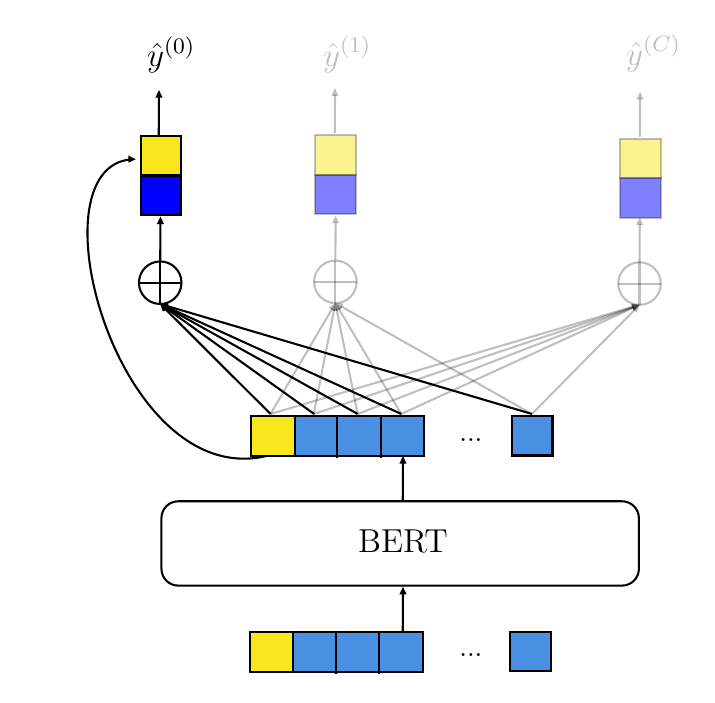
\begin{tikzpicture}[x=0.75pt,y=0.75pt,yscale=-1,xscale=1]
%uncomment if require: \path (0,440); %set diagram left start at 0, and has height of 440

%Straight Lines [id:da31370839057744115] 
\draw [color={rgb, 255:red, 0; green, 0; blue, 0 }  ,draw opacity=0.25 ]   (347.15,213.51) -- (396.86,163.08) ;
\draw [shift={(398.96,160.94)}, rotate = 134.59] [fill={rgb, 255:red, 0; green, 0; blue, 0 }  ,fill opacity=0.25 ][line width=0.08]  [draw opacity=0] (3.57,-1.72) -- (0,0) -- (3.57,1.72) -- cycle    ;
%Straight Lines [id:da20644252238970973] 
\draw [color={rgb, 255:red, 0; green, 0; blue, 0 }  ,draw opacity=0.25 ]   (284.17,213.51) -- (396.24,162.19) ;
\draw [shift={(398.96,160.94)}, rotate = 155.4] [fill={rgb, 255:red, 0; green, 0; blue, 0 }  ,fill opacity=0.25 ][line width=0.08]  [draw opacity=0] (3.57,-1.72) -- (0,0) -- (3.57,1.72) -- cycle    ;

%Straight Lines [id:da4987721771183171] 
\draw [color={rgb, 255:red, 0; green, 0; blue, 0 }  ,draw opacity=0.25 ]   (221.19,213.51) -- (250.92,162.69) ;
\draw [shift={(252.43,160.1)}, rotate = 120.32] [fill={rgb, 255:red, 0; green, 0; blue, 0 }  ,fill opacity=0.25 ][line width=0.08]  [draw opacity=0] (3.57,-1.72) -- (0,0) -- (3.57,1.72) -- cycle    ;
%Straight Lines [id:da39543032652670385] 
\draw [color={rgb, 255:red, 0; green, 0; blue, 0 }  ,draw opacity=0.25 ]   (347.15,213.51) -- (255.04,161.57) ;
\draw [shift={(252.43,160.1)}, rotate = 29.42] [fill={rgb, 255:red, 0; green, 0; blue, 0 }  ,fill opacity=0.25 ][line width=0.08]  [draw opacity=0] (3.57,-1.72) -- (0,0) -- (3.57,1.72) -- cycle    ;
%Straight Lines [id:da4699737293510331] 
\draw [color={rgb, 255:red, 0; green, 0; blue, 0 }  ,draw opacity=0.25 ]   (284.17,213.51) -- (253.96,162.68) ;
\draw [shift={(252.43,160.1)}, rotate = 59.28] [fill={rgb, 255:red, 0; green, 0; blue, 0 }  ,fill opacity=0.25 ][line width=0.08]  [draw opacity=0] (3.57,-1.72) -- (0,0) -- (3.57,1.72) -- cycle    ;
%Straight Lines [id:da5997958802161731] 
\draw [color={rgb, 255:red, 0; green, 0; blue, 0 }  ,draw opacity=0.25 ]   (263.18,213.51) -- (253.02,163.04) ;
\draw [shift={(252.43,160.1)}, rotate = 78.62] [fill={rgb, 255:red, 0; green, 0; blue, 0 }  ,fill opacity=0.25 ][line width=0.08]  [draw opacity=0] (3.57,-1.72) -- (0,0) -- (3.57,1.72) -- cycle    ;
%Straight Lines [id:da30720230167335916] 
\draw [color={rgb, 255:red, 0; green, 0; blue, 0 }  ,draw opacity=0.25 ]   (241.98,213.72) -- (251.86,163.04) ;
\draw [shift={(252.43,160.1)}, rotate = 101.03] [fill={rgb, 255:red, 0; green, 0; blue, 0 }  ,fill opacity=0.25 ][line width=0.08]  [draw opacity=0] (3.57,-1.72) -- (0,0) -- (3.57,1.72) -- cycle    ;

%Rounded Rect [id:dp9909194303175699] 
\draw   (168.63,263.71) .. controls (168.63,259.22) and (172.26,255.58) .. (176.75,255.58) -- (390.53,255.58) .. controls (395.02,255.58) and (398.66,259.22) .. (398.66,263.71) -- (398.66,288.09) .. controls (398.66,292.58) and (395.02,296.22) .. (390.53,296.22) -- (176.75,296.22) .. controls (172.26,296.22) and (168.63,292.58) .. (168.63,288.09) -- cycle ;
%Shape: Ellipse [id:dp8846878696918459] 
\draw   (157.79,150.27) .. controls (157.79,144.62) and (162.38,140.03) .. (168.04,140.03) .. controls (173.7,140.03) and (178.28,144.62) .. (178.28,150.27) .. controls (178.28,155.93) and (173.7,160.52) .. (168.04,160.52) .. controls (162.38,160.52) and (157.79,155.93) .. (157.79,150.27) -- cycle ;
%Straight Lines [id:da9716398351717932] 
\draw    (157.79,150.27) -- (178.28,150.27) ;
%Straight Lines [id:da6639959454699502] 
\draw    (168.04,140.03) -- (168.04,160.52) ;

%Shape: Ellipse [id:dp6966965234878091] 
\draw  [color={rgb, 255:red, 0; green, 0; blue, 0 }  ,draw opacity=0.25 ] (388.72,150.69) .. controls (388.72,145.04) and (393.31,140.45) .. (398.96,140.45) .. controls (404.62,140.45) and (409.21,145.04) .. (409.21,150.69) .. controls (409.21,156.35) and (404.62,160.94) .. (398.96,160.94) .. controls (393.31,160.94) and (388.72,156.35) .. (388.72,150.69) -- cycle ;
%Straight Lines [id:da26514083245396947] 
\draw [color={rgb, 255:red, 0; green, 0; blue, 0 }  ,draw opacity=0.25 ]   (388.72,150.69) -- (409.21,150.69) ;
%Straight Lines [id:da26578756686682437] 
\draw [color={rgb, 255:red, 0; green, 0; blue, 0 }  ,draw opacity=0.25 ]   (398.96,140.45) -- (398.96,160.94) ;

%Shape: Ellipse [id:dp6253805887233457] 
\draw  [color={rgb, 255:red, 0; green, 0; blue, 0 }  ,draw opacity=0.25 ] (242.19,149.86) .. controls (242.19,144.2) and (246.77,139.61) .. (252.43,139.61) .. controls (258.09,139.61) and (262.68,144.2) .. (262.68,149.86) .. controls (262.68,155.51) and (258.09,160.1) .. (252.43,160.1) .. controls (246.77,160.1) and (242.19,155.51) .. (242.19,149.86) -- cycle ;
%Straight Lines [id:da7602382209259668] 
\draw [color={rgb, 255:red, 0; green, 0; blue, 0 }  ,draw opacity=0.25 ]   (242.19,149.86) -- (262.68,149.86) ;
%Straight Lines [id:da0674775185762857] 
\draw [color={rgb, 255:red, 0; green, 0; blue, 0 }  ,draw opacity=0.25 ]   (252.43,139.61) -- (252.43,160.1) ;

%Curve Lines [id:da19895538466908347] 
\draw    (221.19,233.24) .. controls (148.43,253.65) and (104.68,95.04) .. (153.94,90.85) ;
\draw [shift={(156.25,90.77)}, rotate = 180.65] [fill={rgb, 255:red, 0; green, 0; blue, 0 }  ][line width=0.08]  [draw opacity=0] (3.57,-1.72) -- (0,0) -- (3.57,1.72) -- cycle    ;
%Straight Lines [id:da9633912521103427] 
\draw    (221.19,213.51) -- (170.16,162.64) ;
\draw [shift={(168.04,160.52)}, rotate = 44.91] [fill={rgb, 255:red, 0; green, 0; blue, 0 }  ][line width=0.08]  [draw opacity=0] (3.57,-1.72) -- (0,0) -- (3.57,1.72) -- cycle    ;
%Straight Lines [id:da9462664491194832] 
\draw    (242.19,213.51) -- (170.48,162.26) ;
\draw [shift={(168.04,160.52)}, rotate = 35.55] [fill={rgb, 255:red, 0; green, 0; blue, 0 }  ][line width=0.08]  [draw opacity=0] (3.57,-1.72) -- (0,0) -- (3.57,1.72) -- cycle    ;
%Straight Lines [id:da5464988488704245] 
\draw    (263.18,213.51) -- (170.66,161.98) ;
\draw [shift={(168.04,160.52)}, rotate = 29.11] [fill={rgb, 255:red, 0; green, 0; blue, 0 }  ][line width=0.08]  [draw opacity=0] (3.57,-1.72) -- (0,0) -- (3.57,1.72) -- cycle    ;
%Straight Lines [id:da7029151753238021] 
\draw    (284.17,213.51) -- (170.77,161.76) ;
\draw [shift={(168.04,160.52)}, rotate = 24.53] [fill={rgb, 255:red, 0; green, 0; blue, 0 }  ][line width=0.08]  [draw opacity=0] (3.57,-1.72) -- (0,0) -- (3.57,1.72) -- cycle    ;
%Straight Lines [id:da8906632189256127] 
\draw    (347.15,213.51) -- (170.91,161.37) ;
\draw [shift={(168.04,160.52)}, rotate = 16.48] [fill={rgb, 255:red, 0; green, 0; blue, 0 }  ][line width=0.08]  [draw opacity=0] (3.57,-1.72) -- (0,0) -- (3.57,1.72) -- cycle    ;
%Shape: Rectangle [id:dp3507359402768697] 
\draw  [fill={rgb, 255:red, 248; green, 231; blue, 28 }  ,fill opacity=1 ] (158.63,79.57) -- (178.2,79.57) -- (178.2,98.63) -- (158.63,98.63) -- cycle ;
%Shape: Rectangle [id:dp03364773196100135] 
\draw  [fill={rgb, 255:red, 0; green, 0; blue, 255 }  ,fill opacity=1 ] (158.63,98.63) -- (178.2,98.63) -- (178.2,117.69) -- (158.63,117.69) -- cycle ;
%Shape: Rectangle [id:dp46210527300453075] 
\draw  [fill={rgb, 255:red, 74; green, 144; blue, 226 }  ,fill opacity=1 ] (232.11,318.36) -- (294.46,318.36) -- (294.46,337.96) -- (232.11,337.96) -- cycle ;
%Straight Lines [id:da2128074768126642] 
\draw    (252.61,318.5) -- (252.61,338.56) ;
%Shape: Rectangle [id:dp6487133382547166] 
\draw  [fill={rgb, 255:red, 74; green, 144; blue, 226 }  ,fill opacity=1 ] (336.66,318.47) -- (356.22,318.47) -- (356.22,337.54) -- (336.66,337.54) -- cycle ;
%Straight Lines [id:da7615394976975725] 
\draw    (273.61,318.5) -- (273.61,338.56) ;
%Shape: Rectangle [id:dp05494384978133815] 
\draw  [fill={rgb, 255:red, 248; green, 231; blue, 28 }  ,fill opacity=1 ] (211.12,318.36) -- (232.11,318.36) -- (232.11,337.93) -- (211.12,337.93) -- cycle ;

%Straight Lines [id:da42222888162050465] 
\draw [color={rgb, 255:red, 0; green, 0; blue, 0 }  ,draw opacity=0.25 ]   (242.19,213.51) -- (396.12,161.89) ;
\draw [shift={(398.96,160.94)}, rotate = 161.46] [fill={rgb, 255:red, 0; green, 0; blue, 0 }  ,fill opacity=0.25 ][line width=0.08]  [draw opacity=0] (3.57,-1.72) -- (0,0) -- (3.57,1.72) -- cycle    ;
%Straight Lines [id:da6024765910505723] 
\draw [color={rgb, 255:red, 0; green, 0; blue, 0 }  ,draw opacity=0.25 ]   (221.19,213.51) -- (396.09,161.79) ;
\draw [shift={(398.96,160.94)}, rotate = 163.53] [fill={rgb, 255:red, 0; green, 0; blue, 0 }  ,fill opacity=0.25 ][line width=0.08]  [draw opacity=0] (3.57,-1.72) -- (0,0) -- (3.57,1.72) -- cycle    ;
%Straight Lines [id:da7725736479801701] 
\draw [color={rgb, 255:red, 0; green, 0; blue, 0 }  ,draw opacity=0.25 ]   (263.18,213.51) -- (396.17,162.02) ;
\draw [shift={(398.96,160.94)}, rotate = 158.84] [fill={rgb, 255:red, 0; green, 0; blue, 0 }  ,fill opacity=0.25 ][line width=0.08]  [draw opacity=0] (3.57,-1.72) -- (0,0) -- (3.57,1.72) -- cycle    ;
%Straight Lines [id:da8868304751030796] 
\draw    (284.89,255.43) -- (285,236.84) ;
\draw [shift={(285.01,233.84)}, rotate = 90.32] [fill={rgb, 255:red, 0; green, 0; blue, 0 }  ][line width=0.08]  [draw opacity=0] (3.57,-1.72) -- (0,0) -- (3.57,1.72) -- cycle    ;
%Straight Lines [id:da6008487533551252] 
\draw    (284.89,318.41) -- (285,299.82) ;
\draw [shift={(285.01,296.82)}, rotate = 90.32] [fill={rgb, 255:red, 0; green, 0; blue, 0 }  ][line width=0.08]  [draw opacity=0] (3.57,-1.72) -- (0,0) -- (3.57,1.72) -- cycle    ;
%Straight Lines [id:da899337147902147] 
\draw    (168.04,140.03) -- (168.14,121.44) ;
\draw [shift={(168.16,118.44)}, rotate = 90.32] [fill={rgb, 255:red, 0; green, 0; blue, 0 }  ][line width=0.08]  [draw opacity=0] (3.57,-1.72) -- (0,0) -- (3.57,1.72) -- cycle    ;
%Straight Lines [id:da8507680199625551] 
\draw [color={rgb, 255:red, 0; green, 0; blue, 0 }  ,draw opacity=0.25 ]   (252.43,139.61) -- (252.53,121.02) ;
\draw [shift={(252.55,118.02)}, rotate = 90.32] [fill={rgb, 255:red, 0; green, 0; blue, 0 }  ,fill opacity=0.25 ][line width=0.08]  [draw opacity=0] (3.57,-1.72) -- (0,0) -- (3.57,1.72) -- cycle    ;
%Straight Lines [id:da1747682258222547] 
\draw [color={rgb, 255:red, 0; green, 0; blue, 0 }  ,draw opacity=0.25 ]   (398.96,140.45) -- (399.07,121.86) ;
\draw [shift={(399.08,118.86)}, rotate = 90.32] [fill={rgb, 255:red, 0; green, 0; blue, 0 }  ,fill opacity=0.25 ][line width=0.08]  [draw opacity=0] (3.57,-1.72) -- (0,0) -- (3.57,1.72) -- cycle    ;
%Straight Lines [id:da05436810298257799] 
\draw    (167.33,79.09) -- (167.43,60.5) ;
\draw [shift={(167.45,57.5)}, rotate = 90.32] [fill={rgb, 255:red, 0; green, 0; blue, 0 }  ][line width=0.08]  [draw opacity=0] (3.57,-1.72) -- (0,0) -- (3.57,1.72) -- cycle    ;
%Shape: Rectangle [id:dp9332326457526785] 
\draw  [color={rgb, 255:red, 0; green, 0; blue, 0 }  ,draw opacity=0.25 ][fill={rgb, 255:red, 248; green, 231; blue, 28 }  ,fill opacity=0.5 ] (242.61,79.15) -- (262.17,79.15) -- (262.17,98.21) -- (242.61,98.21) -- cycle ;
%Shape: Rectangle [id:dp43512567814545333] 
\draw  [color={rgb, 255:red, 0; green, 0; blue, 0 }  ,draw opacity=0.25 ][fill={rgb, 255:red, 0; green, 0; blue, 255 }  ,fill opacity=0.5 ] (242.61,98.21) -- (262.17,98.21) -- (262.17,117.27) -- (242.61,117.27) -- cycle ;
%Shape: Rectangle [id:dp31911680926128727] 
\draw  [color={rgb, 255:red, 0; green, 0; blue, 0 }  ,draw opacity=0.25 ][fill={rgb, 255:red, 248; green, 231; blue, 28 }  ,fill opacity=0.5 ] (389.56,80.83) -- (409.13,80.83) -- (409.13,99.89) -- (389.56,99.89) -- cycle ;
%Shape: Rectangle [id:dp8655767183794414] 
\draw  [color={rgb, 255:red, 0; green, 0; blue, 0 }  ,draw opacity=0.25 ][fill={rgb, 255:red, 0; green, 0; blue, 255 }  ,fill opacity=0.5 ] (389.56,99.89) -- (409.13,99.89) -- (409.13,118.95) -- (389.56,118.95) -- cycle ;
%Straight Lines [id:da16085998336579554] 
\draw [color={rgb, 255:red, 0; green, 0; blue, 0 }  ,draw opacity=0.25 ]   (252.14,78.25) -- (252.25,59.66) ;
\draw [shift={(252.26,56.66)}, rotate = 90.32] [fill={rgb, 255:red, 0; green, 0; blue, 0 }  ,fill opacity=0.25 ][line width=0.08]  [draw opacity=0] (3.57,-1.72) -- (0,0) -- (3.57,1.72) -- cycle    ;
%Straight Lines [id:da007094542952027716] 
\draw [color={rgb, 255:red, 0; green, 0; blue, 0 }  ,draw opacity=0.25 ]   (399.1,79.93) -- (399.2,61.34) ;
\draw [shift={(399.22,58.34)}, rotate = 90.32] [fill={rgb, 255:red, 0; green, 0; blue, 0 }  ,fill opacity=0.25 ][line width=0.08]  [draw opacity=0] (3.57,-1.72) -- (0,0) -- (3.57,1.72) -- cycle    ;
%Shape: Rectangle [id:dp20108523415186186] 
\draw  [fill={rgb, 255:red, 74; green, 144; blue, 226 }  ,fill opacity=1 ] (232.91,214.36) -- (295.26,214.36) -- (295.26,233.96) -- (232.91,233.96) -- cycle ;
%Straight Lines [id:da9290869404007094] 
\draw    (253.41,214.5) -- (253.41,234.56) ;
%Shape: Rectangle [id:dp43464943110250087] 
\draw  [fill={rgb, 255:red, 74; green, 144; blue, 226 }  ,fill opacity=1 ] (337.46,214.47) -- (357.02,214.47) -- (357.02,233.54) -- (337.46,233.54) -- cycle ;
%Straight Lines [id:da5647307718463164] 
\draw    (274.41,214.5) -- (274.41,234.56) ;
%Shape: Rectangle [id:dp658752958965878] 
\draw  [fill={rgb, 255:red, 248; green, 231; blue, 28 }  ,fill opacity=1 ] (211.92,214.36) -- (232.91,214.36) -- (232.91,233.93) -- (211.92,233.93) -- cycle ;


% Text Node
\draw (158.52,28.5) node [anchor=north west][inner sep=2pt]  [font=\large] [align=left] {$\displaystyle \hat{y}^{( 0)}$};
% Text Node
\draw (285,275) node [anchor=center][inner sep=2pt]  [font=\large] [align=left] {{BERT}};
% Text Node
\draw (243.32,28.3) node [anchor=north west][inner sep=2pt]  [font=\large,color={rgb, 255:red, 0; green, 0; blue, 0 }  ,opacity=0.25 ] [align=left] {$\displaystyle \hat{y}^{( 1)}$};
% Text Node
\draw (389.32,27.9) node [anchor=north west][inner sep=2pt]  [font=\large,color={rgb, 255:red, 0; green, 0; blue, 0 }  ,opacity=0.25 ] [align=left] {$\displaystyle \hat{y}^{( C)}$};
% Text Node
\draw (309,222) node [anchor=north west][inner sep=2pt]   [align=left] {...};
% Text Node
\draw (309,326) node [anchor=north west][inner sep=2pt]   [align=left] {...};

\end{tikzpicture}
\end{center}

\caption{Visualization of the label-aware attention mechanism. The yellow block corresponds to the \texttt{[CLS]} token or its vector representation $\hv_1$.}
\label{fig:model}
\end{figure}

\subsection{Label-Aware Attention}

Given a tokenized text sequence $\xv$ of length $L$, we first obtain its contextualized representation from a pretrained language model: $\Hv = [\hv_1 \hv_2 \cdots \hv_L]^T \in \Rb^{L \times d}$, where $\hv_i$ is a $d$-dimensional vector representation for $i$-th token. 

For an emotion $i$, we maintain a trainable representation $\ev^{(i)} \in \Rb^{d'}$ and use it to query $\Hv$, where the attention scores are computed by bilinear products via a trainable matrix $\Wv \in \Rb^{d' \times d}$ to help align vector space of $\{\ev^{(i)}\}_{i = 1}^C$ and $\{\hv_j\}_{j = 1}^L$. Meanwhile, We omit linear projections of queries, keys and values as in \citet{vaswani2017attention}. A \texttt{softmax} layer is applied to the bilinear products to compute the attention weight distribution, 
$$\alpha_j^{(i)} = \texttt{softmax}\Bigl( \ev^{(i)T}\Wv_{\text{attn}}\hv_j \Bigr) = \frac{\exp(\ev^{(i)T} \Wv_{\text{attn}}  \hv_j)}{\sum_{k = 1}^L \exp(\ev^{(i)T} \Wv_{\text{attn}}  \hv_k)}$$
where $\alpha_j^{(i)}$ denotes the attention weight assigned by emotion $i$ to the $j$-th token. 

Finally, we aggregate the contextualized representations using weights computed above to obtain label-aware sentence representations (as indicated by dark blue boxes in Figure \ref{fig:model}): 
$$\tilde{\hv}^{(i)} = \sum_{k = 1}^L \alpha_k^{(i)} \hv_k.$$

\subsection{Classification Head}

While leveraging label semantics to pool last-layer representations from the pretrained language model, we do not waste the language model's intrinsic ability to extract sentence-level representation. Therefore, for an emotion $i$, we concatenate the label-aware sentence embedding $\tilde{\hv}^{(i)}$ with the typical embedding from \texttt{[CLS]} token $\hv_1$. The concatenated vector is passed into a MLP, which outputs the scalar probability that emotion $i$ exists in the input text: 
$$\hat{y}^{(i)} = \sigma\Bigl( \text{FFN}_i ([\tilde{\hv}^{(i)} \| \hv_1]) \Bigr).$$

We tie weights of classification head $\text{FFN}_{i}$ for all emotion $i$ to encourage the attention module to focus on different sets of contextualized embeddings in $\Hv$. This also prevents the classifier size grows linearly with respect to the number of labels. However, it is possible to inject stronger inductive bias and design specialized head for each label. We leave this idea for future works. 

\subsection{Class-Balanced Loss based on ENS}
In previous error analysis, we found that the baseline model often fails to distinguish low-resourced emotions from high-resourced emotions. This is an issue as the distribution of emotions in the goemotions dataset is unbalanced. To address this issue, we used the class-balanced loss introduced by \citet{cui2019classbalanced}. The effective number of samples (ENS) is defined as 
$
E_c = (1-\beta^{n_c}) / (1-\beta) 
$, where $\beta$ is a hyper-parameter (usually between 0.9 and 1) and $n_c$ is number of samples with emotion $c$. The class-balanced (CB) loss $\mathcal{L}_{CB}(p, y)$ weights the original loss by the ENS as follows:
$$
\mathcal{L}_{CB}(p, y) = \dfrac{1}{E_c} \mathcal{L} (p, y) = \dfrac{1-\beta}{1-\beta^{n_c}}\mathcal{L} (p, y)
$$
where $\mathcal{L} (p, y)$ is the cross entropy loss. 